%%%%%%%%%%%%%%%%%%%%%%%%%%%%%%%%%%%%%%%%%
% University/School Laboratory Report
% LaTeX Template
% Version 3.0 (4/2/13)
%
% This template has been downloaded from:
% http://www.LaTeXTemplates.com
%
% Original author:
% Linux and Unix Users Group at Virginia Tech Wiki 
% (https://vtluug.org/wiki/Example_LaTeX_chem_lab_report)
%
% License:
% CC BY-NC-SA 3.0 (http://creativecommons.org/licenses/by-nc-sa/3.0/)
%
%%%%%%%%%%%%%%%%%%%%%%%%%%%%%%%%%%%%%%%%%

%----------------------------------------------------------------------------------------
%	PACKAGES AND DOCUMENT CONFIGURATIONS
%----------------------------------------------------------------------------------------
\documentclass{article}
\usepackage{amsmath}
\usepackage{amsfonts}
\usepackage{amssymb}
\usepackage{siunitx} % Provides the \SI{}{} command for typesetting SI units
\usepackage{graphicx} % Required for the inclusion of images
\setlength\parindent{0pt} % Removes all indentation from paragraphs
\renewcommand{\labelenumi}{\alph{enumi}.} % Make numbering in the enumerate environment by letter rather than number (e.g. section 6)
\def\thesection{\Alph{section}} % make the secions be index by letters
\usepackage[section]{placeins} % make sure figures are placed in the correct section
\usepackage{pdfpages}
\usepackage[version=3]{mhchem} % chemistry typesetting
%\usepackage{times} % Uncomment to use the Times New Roman font

%----------------------------------------------------------------------------------------
%	DOCUMENT INFORMATION
%----------------------------------------------------------------------------------------
\title{ Pyralis Engine Design \\ MIT Rocket Team} % Title
\author{Matt Vernacchia, President\\James Logan, Vice President\\Connie Liu, Treasurer\\Ben Corbin, Safety Officer
\\\\ Prof. Paulo Lozano, Faculty Advisor} % Author name
\date{ \today } % Date for the report

%----------------------------------------------------------------------------------------
% THE BODY OF THE REPORT
%---------------------------------------------------------------------------------------

\begin{document}
\maketitle
\part*{Engine Design}
\section*{Propellant Selection}
We require propellants which:
\begin{enumerate}
\item Are storable at room temperature (non-cryogenic).
\item Are able to be liquefied at room temperature ($\SI{295}{\kelvin}$) so as to have compact sized tanks.
\item Have a high vapour pressure at room temperature so that the propellants will self-pressurize the combustion chamber. This eliminates the need for a turbopump or inert gas system to pressurize the combustion chamber, greatly simplifying the engine design.
\item Are non-toxic or low-toxicity.
\item Are low-cost and readily available.
\end{enumerate}
Nitrous oxide (\ce{N2O}) is the oxidizer most widely used in hobby rocketry. \ce{N2O} and hydrogen peroxide are the only widely used oxidizer which can be liquid at room temperature, and \ce{N2O} is the less toxic and more stable of the two. \ce{N2O} also presents a vapour pressure of $\SI{5.29}{\mega\pascal}$ at $\SI{295}{\kelvin}$, which is a sufficient combustion chamber pressure. Thus \ce{N2O} will be our oxidizer.\\
\begin{figure}[h!]
\centering
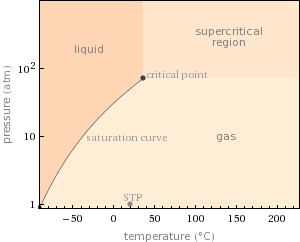
\includegraphics[width = 0.8\textwidth]{n2o_vap.png}
\caption{Vapour pressure curve of nitrous oxide} 
\label{n2o_vap}
\end{figure}
Alkane hydrocarbon fuels provide a high energy density and are comparatively cheap. All alkanes but methane (\ce{CH4}) can be liquefied at room temperature. Of these, ethane (\ce{C2H6}) presents the highest vapour pressure of $\SI{4.40}{\mega\pascal}$. Ethane has a similar vapour pressure curve and critical point to \ce{N2O}, making a convenient pairing. Therefore we will use ethane as our fuel.
\begin{figure}[h!]
\centering
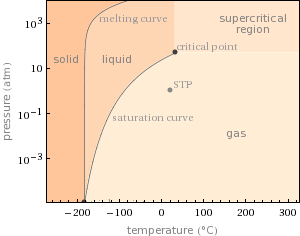
\includegraphics[width = 0.8\textwidth]{c2h6_vap.png}
\caption{Vapour pressure curve of ethane} 
\label{c2h6_vap}
\end{figure}
We will use a oxidizer to fuel ratio of $3:1$ by mass. This ratio is fuel-rich compared to the stoichiometric ratio. NASA's CEARUN tool predicts that this mixture will yield an adiabatic flame temperature of $\SI{1727}{K}$ \cite{CEARUN}. CEARUN tool also predicts that the fuel-rich burn will produce significant amounts of hydrogen ($0.41$ mole fraction), and carbon monoxide ( $0.27$ mole fraction). A oxidizer-rich burn would produce significant nitrogen and carbon dioxide by-products. As \ce{H2} and \ce{CO} are of lower molar mass than \ce{N2} and \ce{CO2}, a fuel-rich burn will produce lower exhaust molar mass and therefore higher specific impulse than an oxidizer-rich combustion process.
\section*{Engine Requirements}
The objective of the Pyralis engine is to boost a rocket vehicle carrying a $\SI{4.5}{\kg}$ payload to an altitude of $\SI{3050}{\metre}$, which is the mission specified by the Intercollegiate Rocket Engineering Competition (IREC). Given the selected propellant ratio,  the structural mass of previous rockets built by the team, a $\SI{3}{\kg}$ engine and $\SI{2}{\kg}$ of plumbing and valves, we predict a total un-fueled rocket mass of $\SI{17}{\kg}$. Based on CEARUN's results, we assume a conservative $I_{sp}$ of $\SI{290}{\second}$. 
Given these assumptions, we perform a simulation of the vehicle's flight to determine the mass of propellant required to lift the vehicle to the target altitude. Our simulation assumes the rocket travels only in the vertical direction and accounts for the effects of aerodynamic drag and gravity. We find that $\SI{3}{\kg}$ of propellant is required for the mission.
\begin{figure}[h!]
\centering
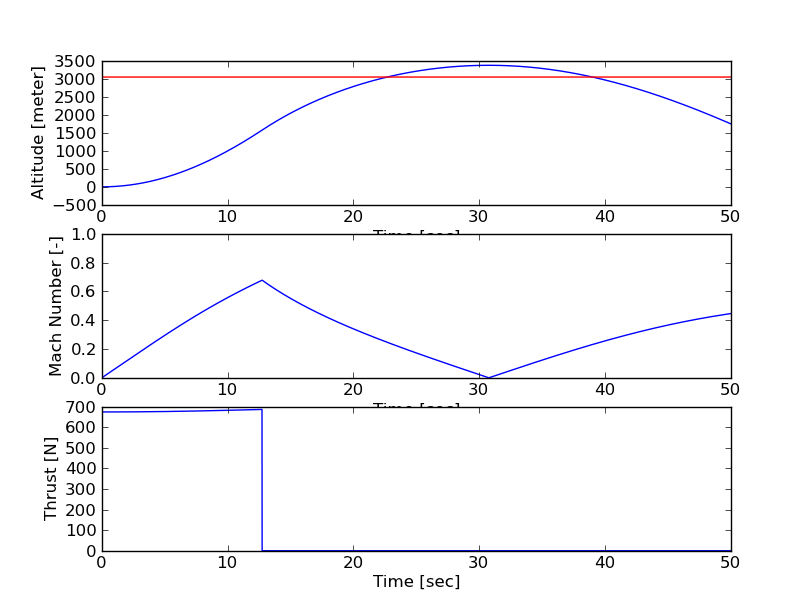
\includegraphics[width = 0.8\textwidth]{ascent_er12.png}
\caption{Simulated Rocket Vehicle Ascent with $\SI{3}{\kg}$ of propellant and $\SI{17}{kg}$ of inert mass} 
\label{ascent}
\end{figure}
For safe launch from a launch rail, we impose that the vehicle must have a take-off thrust to weight ratio of $3.5$ or more. Therefore the engine must provide at least $\SI{20}{\kg} \times \SI{9.8}{\metre\per\second\squared} \times 3.5 = \SI{686}{N}$.\\
To summarize, we require that the engine:
\begin{enumerate}
\item Shall mass less than $\SI{3}{\kg}$.
\item Shall connect to the propellant tanks with plumbing massing less than $\SI{2}{\kg}$
\item Shall have a specific impulse of grater than $\SI{290}{\second}$.
\item Shall produce more than $\SI{686}{N}$ of thrust.
\end{enumerate}
Our simulation indicates that an engine which meets or exceeds these requirements will be able to perform the IREC mission.

\section*{Aerospike Nozzle}
Our engine will use an aerospike, an altitude-compensating nozzle featuring an annular expansion region with an inner solid boundary and an outer fluid boundary. As few aerospike nozzle engines have been produced (excepting the XRS-2200), creating and testing an aerospike engine would allow the team to make a real contribution to the cutting edge of aerospace engineering. A major difficulty with aerospike engines is cooling the spike. However at this small scale we can produce the spike from a material (i.e. graphite or ceramic) which can survive prolonged exposure to the temperature of our exhaust gas without the need for cooling. This eliminates the main factor which would make the use of an aerospike nozzle more difficult that the use of a De Laval nozzle.\\
\begin{figure}[h!]
\centering
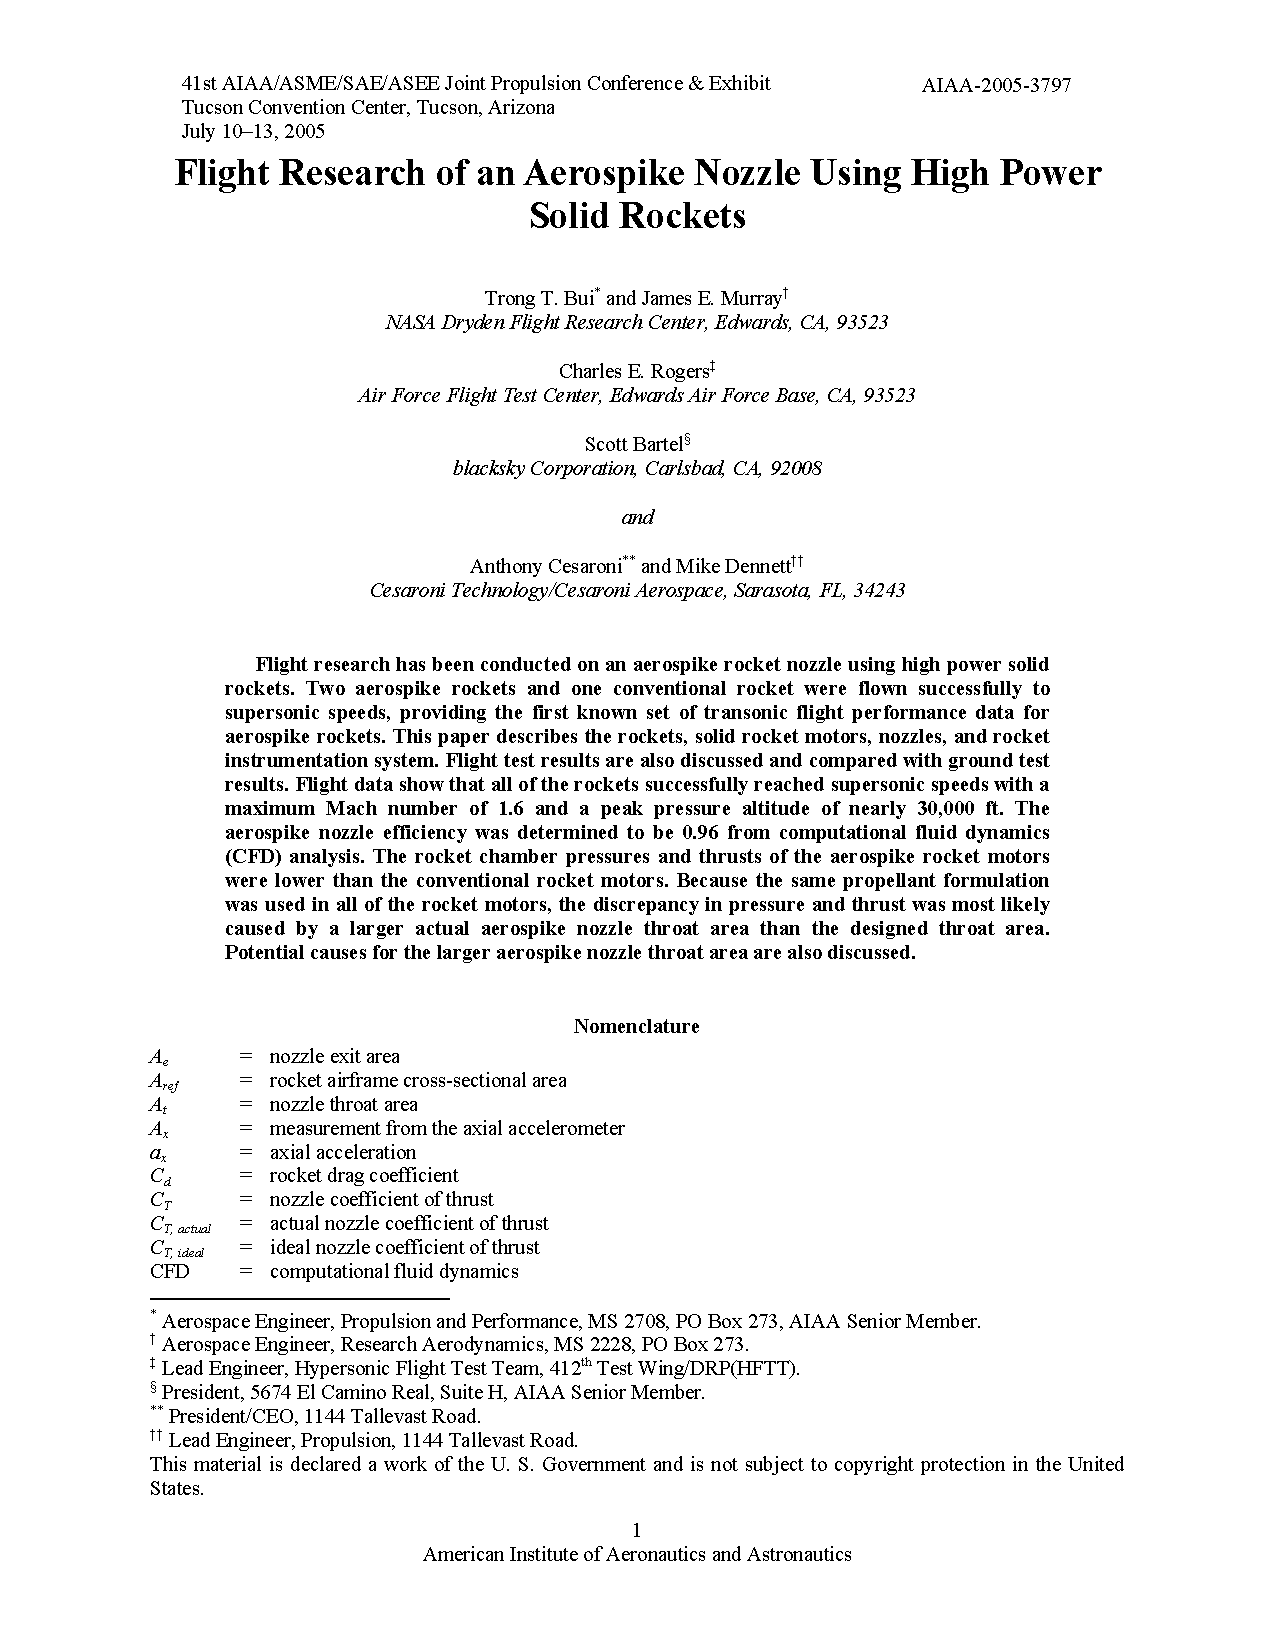
\includegraphics[width = 0.8\textwidth]{dryden_aerospike.png}
\caption{A small aerospike nozzle engine made by NASA Dryden} 
\label{dryden_aerospike}
\end{figure}
C.C. Lee \cite{CCLee} presents a modified method-of-characteristics algorithm for designing the contour of an aerospike nozzle and predicting the performance of the associated engine. There is a revolved Prandtl-Meyer expansion fan emanating from the shroud of the nozzle. For a set of characteristics in the expansion fan, we find the area that each characteristic must have so that the mass flow through each characteristic matches the mass flow at the throat. The algorithm proceeds as follows:
\begin{enumerate}
\item find the Mach number at the exit plane of the engine (the tip of the spike) from the expansion ratio. CC Lee uses a numerical technique to do this, we use an explicit inversion of Stodola's Area-Mach equation.
\item Find the pressure, temperature, and velocity of the fluid at the throat of the nozzle. Use these to find the mass flow rate through the throat.
\item For a range of Mach numbers from 1 to the exit Mach number:
\subitem Find the turn angle of the revolved expansion fan when the flow reaches this Mach number using the Prandtl-Meyer function.
\subitem Find the velocity and density of the fluid at this expansion step.
\subitem The mass flow through each characteristic in the expansion fan must equal the mass flow through the throat. Use this fact to fix the area that this characteristic must have. 
\subitem This characteristic defines a frustum spanning from the throat to some ring on the spike. Use the area and the angle of the characteristic to fix where the bottom ring of the characteristic's frustum must be. This gives the radius of the spike contour must be at a particular axial distance down from the throat.
\end{enumerate} 
For each Mach number examined, the algorithm generates a $(radius, axial distance)$ pair defining a point in cylindrical coordinates through which the spike contour must past. If the algorithm examines enough Mach numbers, the points will trace out a smooth contour line for the plug.\\
Using his algorithm, we predict a thrust of approximately $\SI{715}{\newton}$ and a specific impulse of $\SI{309}{sec}$ for a $\SI{30}{\milli\metre}$ diameter nozzle with expansion ratio $A_e/A_t = 12$ (Fig \ref{spike_contour}).
\begin{figure}[h!]
\centering
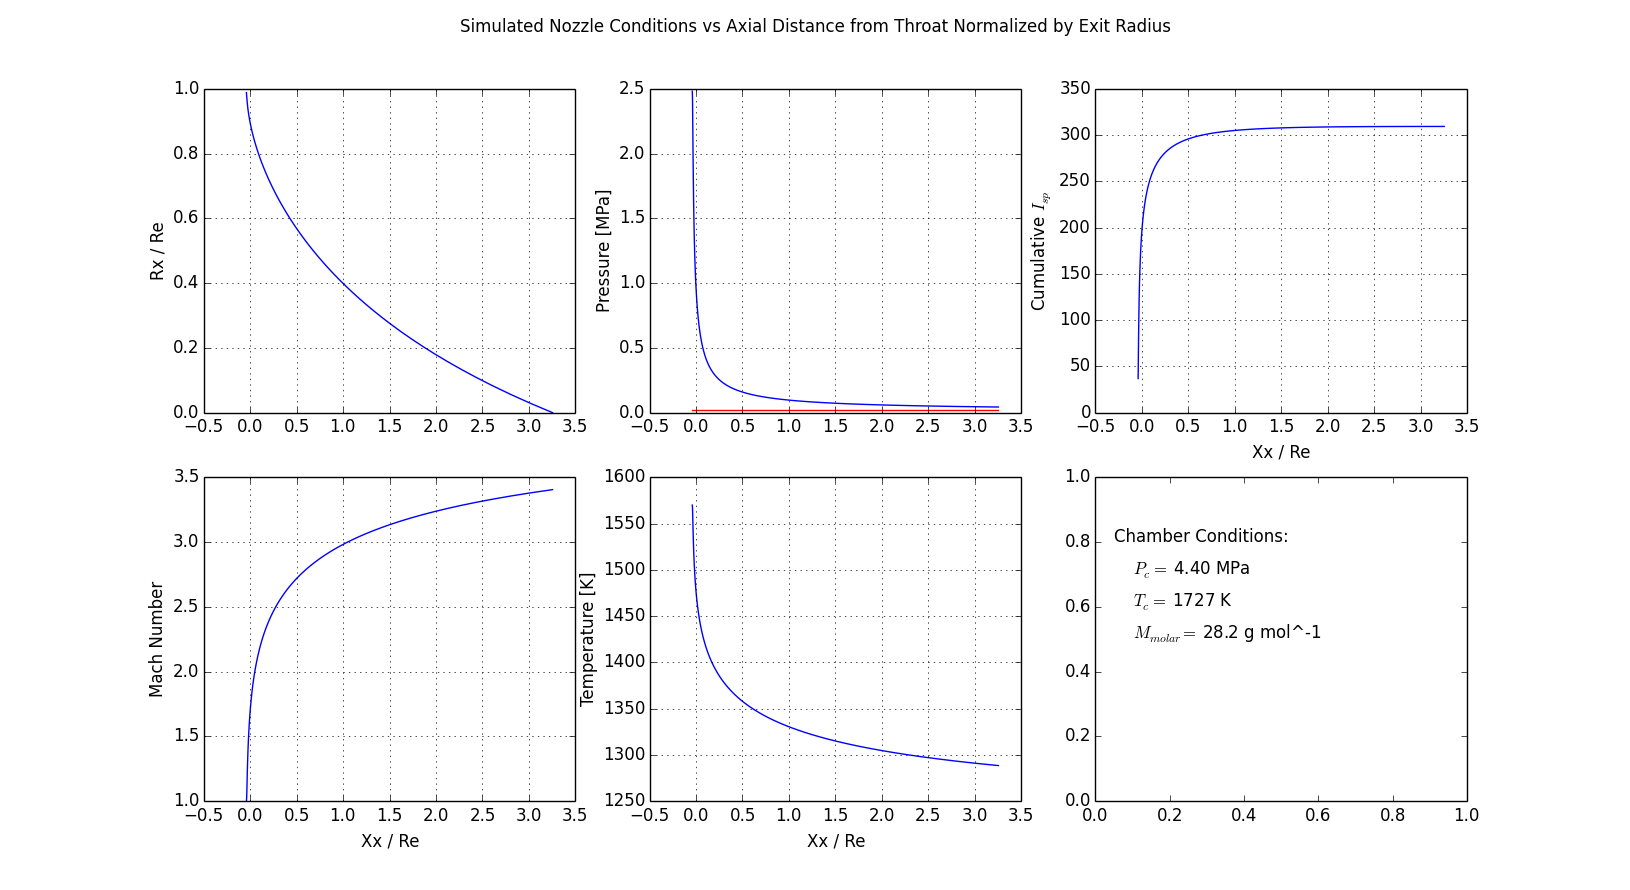
\includegraphics[width = \textwidth]{spike_contour_output.png}
\label{spike_contour}
\end{figure}

\section*{Thermal}
We considered several strategies for keeping the structural elements of the engine sufficiently cool: regenerative cooling, insulating the combustion chamber walls with a layer of un-combusted fuel, and insulating the walls with a ceramic liner. We thought the insulating ceramic to be the easiest to manufacture and analyse, and developed a simulation software to predict its performance. In Fig \ref{thermal}, we see that only $\SI{8}{\milli\metre}$ of insulation is sufficient to keep the wall below $\SI{350}{\kelvin}$. A thinner insulator would be thermodynamically feasible, but would be too difficult to manufacture.
\begin{figure}[h!]
\centering
\includegraphics[width = \textwidth]{thermal.png}
\caption{Model of heat transfer through an insulating ceramic liner to the combustion chamber wall. Temperatures are shown for $\SI{2}{\second}$ to $\SI{20}{\second}$ after the start of a burn} 
\label{thermal}
\end{figure}

\section*{Combustion Chamber}
The combustion chamber will be of a toroidal shape (Fig \ref{comb_chamber}). Its inner and outer radii are chosen to be $\SI{10}{\milli\metre}$ and $\SI{24}{\milli\metre}$.
Now, the length of the combustion chamber required for the propellants to fully combust must be found. Sutton (\cite{RPE}) describes the use of the characteristic length $L^*$ to size the length of a combustion chamber. For a combustion chamber of volume $V$ and throat area $A_t$,
\[ L^* = \frac{V}{A_t} \]
The $L^*$ required to fully combust various propellants has been experimentally determined for many propellant chemistries, but not for ethane and nitrous oxide. As most $L^*$ values range from $\SI{0.5}{\metre}$ to $\SI{1.0}{\metre}$, we chose a conservative $L^*$ of $\SI{1.5}{\metre}$ to size our chamber. Writing the volume of the chamber as a function of length $x_{cc}$, we find the required combustion chamber physical length:
\[ L^* = \frac{x_{cc} \pi(r_{cc,outer}^2 - r_{cc,inner}^2)}{A_t}\]
\[ x_{cc} = \frac{L^* A_t }{ \pi(r_{cc,outer}^2 - r_{cc,inner}^2) } \]
\[ x_{cc} = \frac{ \SI{1.5}{\metre} \times \SI{0.00005890}{\metre\squared} }{ \pi((\SI{0.024}{\metre})^2 - (\SI{0.010}{\metre})^2) } = \SI{60.0}{\milli\metre} \]
\begin{figure}[h!]
\centering
\includegraphics[width = 0.8\textwidth]{comb_chamber.png}
\caption{Cross-section of the combustion chamber and nozzle. White material is insulative ceramic, grey material is steel.} 
\label{comb_chamber}
\end{figure}
\section*{Engine Wall Thickness}
The thickness of the engine wall was chosen by way of matching expected combustion chamber hoop stress to 0.2\% yield strength of the material used (316 stainless steel) at a temperature of 1144K (744 degrees higher than what the steel is expected to encounter) before applying a safety factor of 2. Using the thin walled simplification of the hoop stress calculation:\\
\\
$ t_{min} = \frac{P*r}{\sigma_{\theta,critical}}$
\\
\\
gives a minimum thickness of 1.28mm. Applying a safety factor of 2 gives a thickness of 2.56mm.

\section*{Ignition System}
\subsection*{Device Description}
The ignition system will be spark-type, and will have a mass of less than 0.2kg in total. It will consist of a bank of at least two capacitors charged to C = 120microFarads and V = 320v. Each capacitor can provide 6.1J of energy on discharge across the spark gap. The capacitors will be charged by a charge pump, and will be capable of repeated discharge at approximately 1/5Hz in the event that the ignition sequence need be repeated.
\subsection*{Selection Process}
A spark-type ignition system was selected after examination of the available literature on the subject of nitrous oxide/hydrocarbon ignition under conditions close to STP. Nitrous oxide/hydrocarbon mixtures appear to have an ignition energy requirement which is insensitive to heating, making a purely thermal system extremely weight-inefficient. Other spark-type systems including flyback transformer-type and high-frequency voltage pump-type were investigated and rejected based on mass, ignition energy, and reliability concerns.
\subsection*{Energy Requirements}
The authors of "Flammability, Ignition Energy and Flame Speed" found that the flammability limits of the nitrous oxide-methane mixture at STP were unaffected by increasing the ignition energy beyond 1J. An order-of-magnitude similarity assumption here, based on the chemical similarity of ethane and methane, led to the decision to provide at least 10J of ignition energy.
\subsection*{Geometry}
The ignitor itself will be a standard internal combustion engine-type spark plug, and will be threaded through the injector plate. The spark gap will be oriented vertically in order to prevent arc wandering.

\section*{Prevention of Common Failure Mode}
The failure mode that is both native to and particularly prevalent in aerospike engines is spike detachment (\cite{Mueller}). If the spike detaches from the injector plate, it will suddenly plug the throat of the combustion chamber, causing a water hammer effect and subsequent rupture of the combustion chamber. We will prevent this by threading a rod of stronger material down the center of the spike and attaching the spike to the injector plate using this threaded rod.



\part*{Cold Flow Test}
\section*{Reason for Cold Flow Test}
A cold flow test will allow us to verify our design methods, particularly where the nozzle geometry is concerned, in an environment where failure of the device will not produce catastrophic results. In addition, the cold flow test will give the team practice with the safety procedures that will allow the fully functional engine to be operated without undue risk to personnel as well as practice with the design and fabrication methods that will be used to produce the fully functional engine.
\section*{Cold-flow Prototype Differences}
The cold-flow prototype differs from the fully functional design in the following ways:
\begin{itemize}
\item Plastic used in place of high-temperature ceramic materials
\item No ignitor
\item Simplified injector plate geometry
\item Pressure sensor inserted into mock-combustion chamber through injector plate
\end{itemize}
\begin{figure}[h!]
\centering
\includegraphics[width = \textwidth]{spike_contour_output_cold.png}
\caption{Performance predictions for the engine at the reduced temperature and pressure of the cold flow test}
\label{spike_contour_cold}
\end{figure}

\section*{Experiment Setup}
Number of measurements: 3\\

The cold flow test will consist primarily of the following components, ordered from upstream to downstream:

\begin{itemize}
\item[1]Compressed Air Cylinder
\item[2]Gas delivery hardware
\subitem $\bullet$ Tubing, regulator, and valves
\item[3]Cold-flow prototype Pyralis engine
\item[4]Test Stand
\item[5]Sensors
\subitem$\bullet$ Pressure and load
\end{itemize}
\begin{figure}[h!]
\centering
\includegraphics[width = 0.8\textwidth]{cold_flow.png}
\caption{A schematic of the cold flow experiment setup.} 
\label{cold_flow}
\end{figure}
\subsection*{Data Collection and Processing}
We will collect pressure data from the gas cylinder as well as from the mock-combustion chamber. Load data will be collected from the test stand. These three measurements in combination with a few strategically chosen assumptions will allow us to determine the thrust, $I_{sp}$, and coefficient of thrust $C_F$:
\begin{enumerate}
\item The chamber pressure $p_c$ and the thrust force $F$ are measured directly.
\item The coefficient of thrust can be found by $C_F = \frac{F}{A_t P_c}$
\item Given the tank pressure $p_t(t)$, and assuming the expansion of the gas out of the tank occurs quickly enough to be adiabatic, we find the mass of gas remaining in the tank as at any time, $m(t)$.
\item Numerically differentiating $m(t)$, we get $ \frac{dm}{dt} = \dot{m}$.
\item Knowing $\dot{m}$, we find $I_{sp} = \frac{F}{\dot{m} g_o}$.
\end{enumerate}
A Schlieren photography rig may be added in order to visually determine shockwave location, which would give insights into quality of expansion. 

\section*{Compressed Air Supply}

\subsection*{Tank Capacity}

\subsection*{Pipe Sizing}
\subsubsection*{Reynolds Number Check}
\begin{figure}[h!]
\centering
\includegraphics[width = 0.8\textwidth]{reynolds_vs_diameter.jpg}
\caption{Reynolds number vs pipe diameter for air flow through a pipe at $\dot{m} = \SI{1.28}{\kg\per\second}$\}} 
\label{reynolds}
\end{figure}
We performed a cursory examination of the Reynolds number of flow through the pipe in order to determine which assumptions we could apply when determining the pressure drop per meter of pipe. This graph illustrates the reason for our choice to assume fully turbulent flow.
\subsubsection*{Pressure drop per meter of pipe}
\begin{figure}[h!]
\centering
\includegraphics[width = 0.8\textwidth]{press_drop_vs_diameter.jpg}
\caption{Reynolds number vs pipe diameter for air flow through a pipe at $\dot{m} = \SI{1.28}{\kg\per\second}$\}} 
\label{press_drop}
\end{figure} 
We used a numerical solution to the Colebrook Formula to retrieve the expected pressure drop per meter of copper pipe. Using 3/8" copper pipe will cause a drop of less than 1 bar per meter, which is sufficient to achieve appropriate chamber pressure.

\section*{Safety for the Cold Flow Test}
Our primary safety concerns are:
\begin{itemize}
\item Failure of cold-flow engine prototype
\item Failure of compressed gas hardware
\end{itemize}
\subsection*{Safety Plan}
We will address both issues by performing the test in a blast chamber which provides adequate isolation of the test personnel from the test rig and compressed gas equipment. We will create a safety checklist for use during setup for each test which will be checked by all test personnel before each test.
\begin{thebibliography}{9}
	\bibitem{CEARUN} CEARUN. \emph{NASA.} http://cearun.grc.nasa.gov/.
	\bibitem{Stodola} J. Majdalani and B. A. Maickie. Explicit Inversion of Stodola's Area-Mach Equation. \emph{University of Tennessee Space Institute.} http://maji.utsi.edu/publications/pdf/HT02\_11.pdf
	\bibitem{CCLee} C.C Lee. FORTRAN Programs for Plug Nozzle Design. \emph{NASA Marshal Space Flight Center.} 1963. http://ia700303.us.archive.org/24/items/nasa\_techdoc\_19630012259/19630012259.pdf.
	\bibitem{316} 316 Stainless Steel. \emph{AK Steel.} http://www.aksteel.com/pdf/markets\_products/stainless/austenitic/316\_316L\_Data\_Bulletin.pdf.
	\bibitem{RPE} George P Sutton and Oscar Biblarz. Rocket Propulsion Elements. 2001.
	\bibitem{mueller} Eric Besnard, Hsun Hu Chen, Tom Mueller, and John Garvey. Design, Manufacturing and Test of a Plug Nozzle Rocket Engine. \emph{California State University Long Beach and Garvey Spacecraft Corporation.} AIAA Joint Propulsion Conference. 2002.
	\bibitem{Borisov} Borisov, et. al. Critical conditions for nitrous oxide ignition. http://link.springer.com/article/10.1134\%2FS1990793109040150\#page-1
	
	\bibitem{DARPA} Roger Hardy. NITROUS OXIDE / HYDROCARBON FUEL ADVANCED CHEMICAL PROPULSION: DARPA CONTRACT OVERVIEW. \emph{Qualis Corporation}  http://tfaws.nasa.gov/TFAWS06/Proceedings/Aerothermal-Propulsion/Papers/TFAWS06-1026\_Paper\_Herdy.pdf
	
	\bibitem{Flam} Pfahl, et. al. Flammability, Ignition Energy and Flame Speed. http://www2.galcit.caltech.edu/EDL/publications/reprints/flimits.pdf
\end{thebibliography}
\end{document}
